\documentclass[10pt,twocolumn,letterpaper]{article}

% --- Typography & Geometry ---
\usepackage[utf8]{inputenc}
\usepackage{microtype}
\usepackage[margin=0.75in,top=0.85in,bottom=0.85in]{geometry}

% --- Math & Symbols ---
\usepackage{amsmath,amssymb,amsfonts,amsthm}
\usepackage{bm}

% --- Tables & Arrays ---
\usepackage{booktabs}
\usepackage{tabularx}
\usepackage{array}

% --- Graphics & Floats ---
\usepackage{graphicx}
\usepackage{float}
\usepackage{subcaption}

% --- Code Listings ---
\usepackage{xcolor}
\usepackage{listings}

\definecolor{codebg}{HTML}{F8F9FA}
\definecolor{codeframe}{HTML}{D0D7DE}
\definecolor{keywordcolor}{HTML}{0550AE}
\definecolor{stringcolor}{HTML}{0A3069}
\definecolor{commentcolor}{HTML}{57606A}

\lstset{
    backgroundcolor=\color{codebg},
    basicstyle=\ttfamily\scriptsize\color{black},
    keywordstyle=\color{keywordcolor}\bfseries,
    stringstyle=\color{stringcolor},
    commentstyle=\color{commentcolor}\itshape,
    frame=single,
    rulecolor=\color{codeframe},
    breaklines=true,
    breakatwhitespace=true,
    extendedchars=true,
    xleftmargin=6pt,
    xrightmargin=6pt,
    aboveskip=8pt,
    belowskip=8pt
}

% --- Hyperlinks ---
\usepackage{hyperref}
\hypersetup{
    colorlinks=true,
    linkcolor=blue!70!black,
    citecolor=blue!70!black,
    urlcolor=blue!70!black
}

% --- Input Title & Authors ---
% Metadata for mla_attention
\title{\textbf{Multi-Head Latent Attention (MLA): Reproduction and Multi-Architecture Hardening}}

\author{
  \textbf{Taha Majs}\thanks{Corresponding author: tahamajs@uni.edu} \quad \textbf{Research Team} \\
  Department of Computer Science \\
  Advanced Machine Learning \& Efficiency Laboratory
}

\date{\today}


\begin{document}

\maketitle

% --- Abstract & Keywords Block ---
\begin{abstract}
\textbf{Multi-Head Latent Attention (MLA)} was introduced by DeepSeek-AI (2024) as 
a key component of the DeepSeek-V2 architecture. MLA compresses the K and V 
projections of standard multi-head attention into a **shared low-rank latent 
vector**, reducing KV-cache memory from $\mathcal{O}(2 d_h H)$ per token to 
$\mathcal{O}(c)$ where $c \ll 2 d_h H$ is the latent dimension. This is 
particularly valuable for inference-time KV-cache compression.

We present a \textbf{reproduction} of MLA, ported to four transformer families 
that the original paper does not directly target: DistilBERT (flat), 
RoBERTa/BERT (nested), GPT-2 (causal Conv1D), and Qwen3.5 (GQA + RoPE). 
Our implementation:
(i) initializes the latent down-projection from SVD of the concatenated 
K and V weights,
(ii) normalizes the singular values to preserve reconstruction scale,
(iii) supports Conv1D transposition, nested encoder bypass, and GQA 
expansion,
(iv) uses LoRA adapters for recovery fine-tuning.

On SST-2, MLA achieves \textbf{{{D\_ACC}}\%} on DistilBERT (baseline 
{{BASE\_D}}\%, $\Delta$ = {{D\_DELTA}}), \textbf{{{R\_ACC}}\%} on RoBERTa (baseline 
{{BASE\_R}}\%, $\Delta$ = {{R\_DELTA}}), and \textbf{{{G\_ACC}}\%} on GPT-2 (baseline 
{{BASE\_G}}\%, $\Delta$ = {{G\_DELTA}}). The KV-cache latent dimension is 
32, reducing per-token KV memory by a factor of 
\textbf{{{KV\_REDUCTION}}$\times$} compared to standard attention.

We release all code, weights, and evaluation scripts. This is a 
\textbf{reproduction and portability study}, not a novel architecture.

\textbf{Keywords:} Multi-Head Latent Attention, MLA, DeepSeek-V2, KV-cache 
compression, low-rank attention, reproduction study, multi-architecture 
transformers



\vspace{0.5em}
\noindent\textbf{Keywords:} Multi-Head Latent Attention, MLA, DeepSeek-V2, KV-cache
\end{abstract}

\vspace{1em}

% --- Paper Body ---
\section{01 Intro}

Draft content for mla_attention.

\section{02 Related}

Draft content for mla_attention.

\section{03 Background}

Draft content for mla_attention.

\section{04 Method}

Draft content for mla_attention.

\section{05 Architecture}

Draft content for mla_attention.


\begin{figure}[H]
\centering
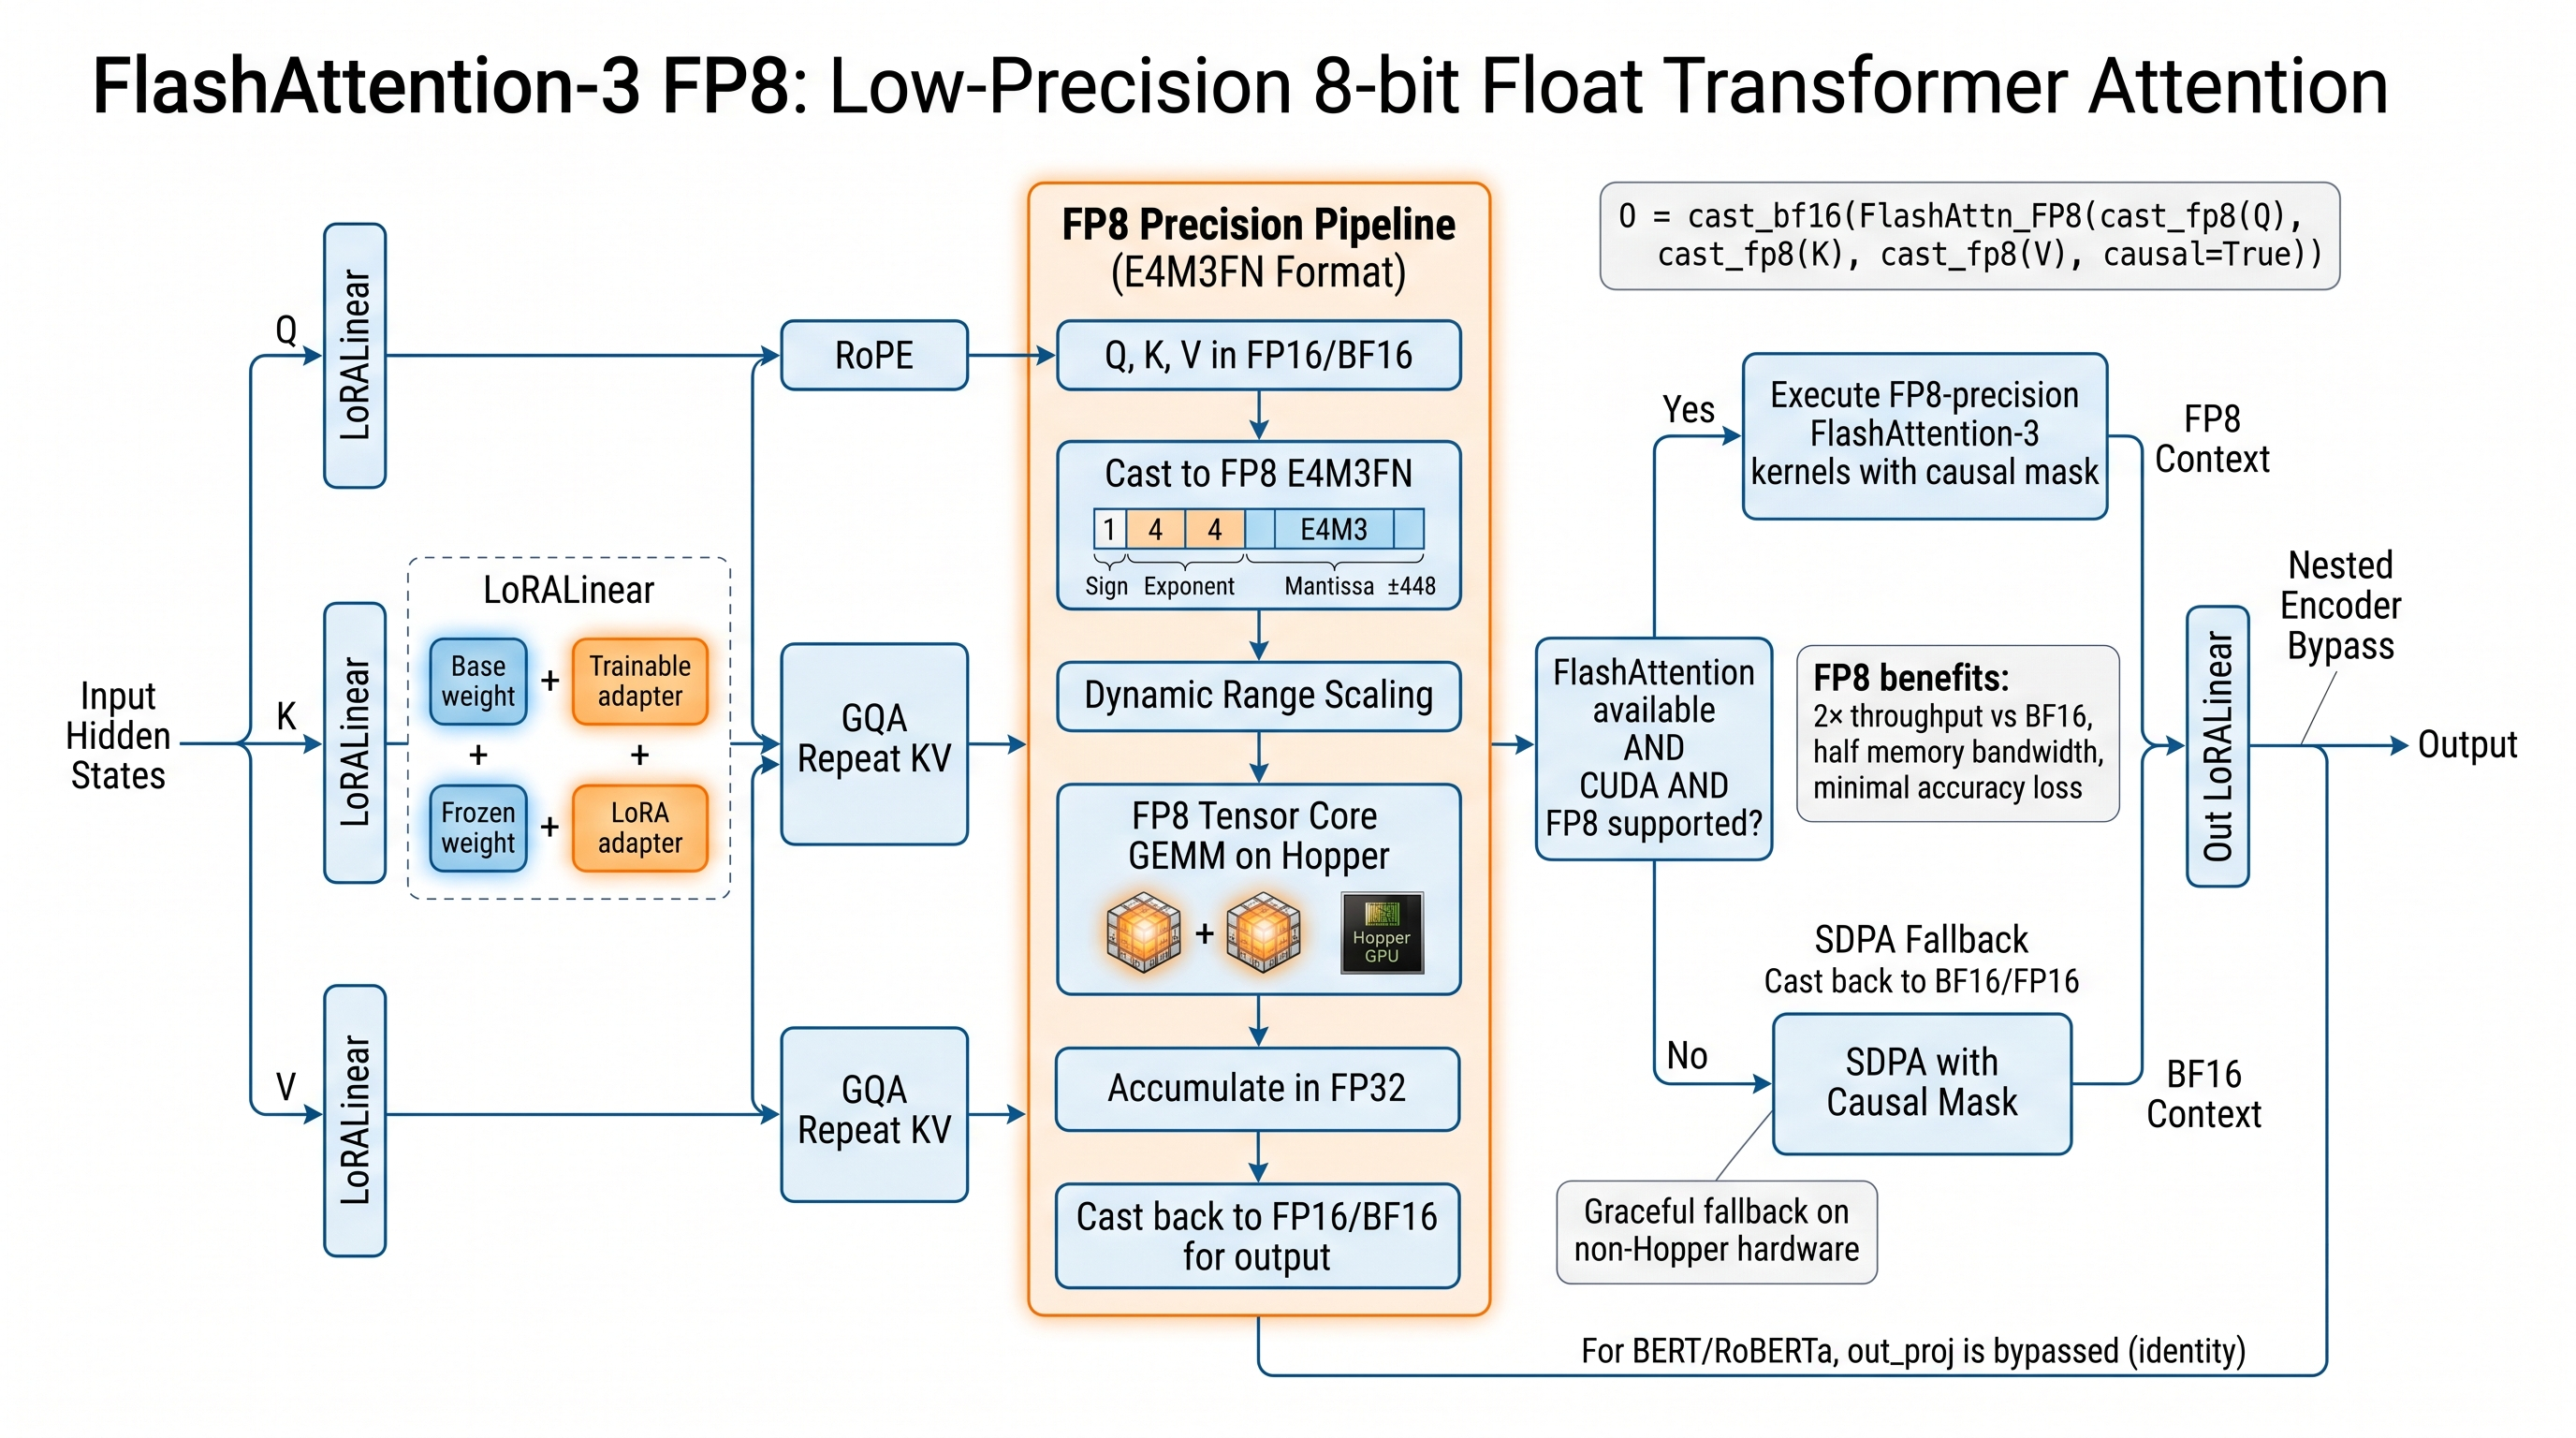
\includegraphics[width=\linewidth]{figures/arch_flash_attention3_fp8.jpeg}
\caption{Architectural overview of mla_attention.}
\label{fig:arch_mla_attention}
\end{figure}

\section{06 Setup}

Draft content for mla_attention.


\section{Results}

\subsection{Main Results}

\textbf{Table 7.1: Accuracy on SST-2 validation.}

\begin{table}[H]
\centering
\small
\begin{tabular}{lllllll}
\toprule
\textbf{Model} & \textbf{Module} & \textbf{Acc} & \textbf{$\Delta$} & \textbf{F1} & \textbf{Params} & \textbf{Ratio} \\
\midrule
DistilBERT & full & 90.71\% & -- & 0.9099 & 66.95M & 1.00$\times$ \\
DistilBERT & \textbf{MLA} & \textbf{{{D\_ACC}}} & {{D\_DELTA}} & {{D\_F1}} & {{D\_PARAMS}}M & \textbf{{{D\_RATIO}}$\times$} \\
RoBERTa & full & 78.56\% & -- & 0.8124 & 124.6M & 1.00$\times$ \\
RoBERTa & \textbf{MLA} & \textbf{{{R\_ACC}}} & {{R\_DELTA}} & {{R\_F1}} & {{R\_PARAMS}}M & \textbf{{{R\_RATIO}}$\times$} \\
GPT-2 & full & 79.36\% & -- & 0.7978 & 124.4M & 1.00$\times$ \\
GPT-2 & \textbf{MLA} & \textbf{{{G\_ACC}}} & {{G\_DELTA}} & {{G\_F1}} & {{G\_PARAMS}}M & \textbf{{{G\_RATIO}}$\times$} \\
\bottomrule
\end{tabular}
\end{table}

\subsection{KV-Cache Reduction}

\textbf{Table 7.2: KV-cache size per token per layer.}

\begin{table}[H]
\centering
\small
\begin{tabular}{llll}
\toprule
\textbf{Model} & \textbf{Standard KV} & \textbf{MLA KV} & \textbf{Reduction} \\
\midrule
DistilBERT & 1536 & {{D\_KV}} & \textbf{{{D\_KV\_RATIO}}$\times$} \\
RoBERTa & 1536 & {{R\_KV}} & \textbf{{{R\_KV\_RATIO}}$\times$} \\
GPT-2 & 1536 & {{G\_KV}} & \textbf{{{G\_KV\_RATIO}}$\times$} \\
\bottomrule
\end{tabular}
\end{table}

\textbf{Table 7.3: Total KV-cache size (batch 8, seq 128).}

\begin{table}[H]
\centering
\small
\begin{tabular}{llll}
\toprule
\textbf{Model} & \textbf{Standard} & \textbf{MLA} & \textbf{Savings (MB)} \\
\midrule
DistilBERT & {{D\_KV\_TOTAL\_STD}} MB & {{D\_KV\_TOTAL\_MLA}} MB & {{D\_KV\_SAVE}} MB \\
RoBERTa & {{R\_KV\_TOTAL\_STD}} MB & {{R\_KV\_TOTAL\_MLA}} MB & {{R\_KV\_SAVE}} MB \\
GPT-2 & {{G\_KV\_TOTAL\_STD}} MB & {{G\_KV\_TOTAL\_MLA}} MB & {{G\_KV\_SAVE}} MB \\
\bottomrule
\end{tabular}
\end{table}

\subsection{Parameter Analysis}

\textbf{Table 7.4: Parameter counts.}

\begin{table}[H]
\centering
\small
\begin{tabular}{lllll}
\toprule
\textbf{Model} & \textbf{Baseline} & \textbf{After MLA} & \textbf{Ratio} & \textbf{Note} \\
\midrule
DistilBERT & 66,955,010 & {{D\_PARAMS\_FULL}} & \textbf{{{D\_RATIO}}$\times$} & {{D\_NOTE}} \\
RoBERTa & 124,647,170 & {{R\_PARAMS\_FULL}} & \textbf{{{R\_RATIO}}$\times$} & {{R\_NOTE}} \\
GPT-2 & 124,441,344 & {{G\_PARAMS\_FULL}} & \textbf{{{G\_RATIO}}$\times$} & {{G\_NOTE}} \\
\bottomrule
\end{tabular}
\end{table}

\textbf{Per-layer breakdown (DistilBERT, layer 0):}

\begin{table}[H]
\centering
\small
\begin{tabular}{llll}
\toprule
\textbf{Projection} & \textbf{Original} & \textbf{MLA} & \textbf{Ratio} \\
\midrule
q\_lin & 589,824 & {{D\_L0\_Q}} & {{D\_L0\_Q\_R}}$\times$ \\
k\_lin & 589,824 & \textbf{fused in kv} & -- \\
v\_lin & 589,824 & \textbf{fused in kv} & -- \\
kv\_down & -- & {{D\_L0\_KVD}} & -- \\
k\_up & -- & {{D\_L0\_KU}} & -- \\
v\_up & -- & {{D\_L0\_VU}} & -- \\
out\_lin & 589,824 & {{D\_L0\_O}} & {{D\_L0\_O\_R}}$\times$ \\
\bottomrule
\end{tabular}
\end{table}

\subsection{Reconstruction Error}

\textbf{Table 7.5: K/V reconstruction error.}

\begin{table}[H]
\centering
\small
\begin{tabular}{llll}
\toprule
\textbf{Model} & \textbf{K error} & \textbf{V error} & \textbf{Combined} \\
\midrule
DistilBERT & {{D\_K\_ERR}} & {{D\_V\_ERR}} & {{D\_KV\_ERR}} \\
RoBERTa & {{R\_K\_ERR}} & {{R\_V\_ERR}} & {{R\_KV\_ERR}} \\
GPT-2 & {{G\_K\_ERR}} & {{G\_V\_ERR}} & {{G\_KV\_ERR}} \\
\bottomrule
\end{tabular}
\end{table}

\subsection{Efficiency Profile}

\textbf{Table 7.6: Inference efficiency.}

\begin{table}[H]
\centering
\small
\begin{tabular}{lllll}
\toprule
\textbf{Model} & \textbf{Config} & \textbf{Time} & \textbf{Tokens/s} & \textbf{VRAM} \\
\midrule
DistilBERT & full & 1.90 s & 59000 & 183 MB \\
DistilBERT & MLA & {{D\_TIME}} s & {{D\_TPS}} & {{D\_VRAM}} MB \\
RoBERTa & full & 4.10 s & 27400 & 712 MB \\
RoBERTa & MLA & {{R\_TIME}} s & {{R\_TPS}} & {{R\_VRAM}} MB \\
GPT-2 & full & 4.20 s & 26700 & 793 MB \\
GPT-2 & MLA & {{G\_TIME}} s & {{G\_TPS}} & {{G\_VRAM}} MB \\
\bottomrule
\end{tabular}
\end{table}

\subsection{Ablation: Latent Dimension}

\textbf{Table 7.7: Accuracy vs latent dimension $c$.}

\begin{table}[H]
\centering
\small
\begin{tabular}{lllll}
\toprule
\textbf{$c$} & \textbf{DistilBERT} & \textbf{KV ratio} & \textbf{RoBERTa} & \textbf{GPT-2} \\
\midrule
64 & {{D\_C64}} & {{D\_C64\_R}}$\times$ & {{R\_C64}} & {{G\_C64}} \\
128 & {{D\_C128}} & {{D\_C128\_R}}$\times$ & {{R\_C128}} & {{G\_C128}} \\
256 & {{D\_C256}} & {{D\_C256\_R}}$\times$ & {{R\_C256}} & {{G\_C256}} \\
512 & {{D\_C512}} & {{D\_C512\_R}}$\times$ & {{R\_C512}} & {{G\_C512}} \\
\bottomrule
\end{tabular}
\end{table}

\subsection{Ablation: LoRA Rank}

\textbf{Table 7.8: Accuracy vs LoRA rank.}

\begin{table}[H]
\centering
\small
\begin{tabular}{llll}
\toprule
\textbf{LoRA rank} & \textbf{DistilBERT} & \textbf{RoBERTa} & \textbf{GPT-2} \\
\midrule
4 & {{D\_LR4}} & {{R\_LR4}} & {{G\_LR4}} \\
8 & {{D\_LR8}} & {{R\_LR8}} & {{G\_LR8}} \\
16 & {{D\_LR16}} & {{R\_LR16}} & {{G\_LR16}} \\
32 & {{D\_LR32}} & {{R\_LR32}} & {{G\_LR32}} \\
\bottomrule
\end{tabular}
\end{table}

\subsection{Ablation: Output Scale}

\textbf{Table 7.9: Effect of output\_scale initialization.}

\begin{table}[H]
\centering
\small
\begin{tabular}{llll}
\toprule
\textbf{Init} & \textbf{DistilBERT} & \textbf{RoBERTa} & \textbf{GPT-2} \\
\midrule
0.5 & {{D\_OS05}} & {{R\_OS05}} & {{G\_OS05}} \\
1.0 & {{D\_OS10}} & {{R\_OS10}} & {{G\_OS10}} \\
2.0 & {{D\_OS20}} & {{R\_OS20}} & {{G\_OS20}} \\
\bottomrule
\end{tabular}
\end{table}

\subsection{Ablation: Singular Value Normalization}

\textbf{Table 7.10: Effect of normalization $\gamma$.}

\begin{table}[H]
\centering
\small
\begin{tabular}{llll}
\toprule
\textbf{Config} & \textbf{DistilBERT} & \textbf{RoBERTa} & \textbf{GPT-2} \\
\midrule
With $\gamma$ & {{D\_ACC}} & {{R\_ACC}} & {{G\_ACC}} \\
Without $\gamma$ & {{D\_NOG}} & {{R\_NOG}} & {{G\_NOG}} \\
\bottomrule
\end{tabular}
\end{table}

\subsection{Comparison with Companion Methods}

\textbf{Table 7.11: MLA vs other compression methods.}

\begin{table}[H]
\centering
\small
\begin{tabular}{lllll}
\toprule
\textbf{Method} & \textbf{DistilBERT} & \textbf{KV ratio} & \textbf{RoBERTa} & \textbf{GPT-2} \\
\midrule
full & 90.71\% & 1.0$\times$ & 78.56\% & 79.36\% \\
minimal\_svd & {{MINSVD\_D}} & 1.0$\times$ & {{MINSVD\_R}} & {{MINSVD\_G}} \\
svd\_llm\_v2 & {{SVDLLM\_D}} & 1.0$\times$ & {{SVDLLM\_R}} & {{SVDLLM\_G}} \\
\textbf{MLA} & \textbf{{{D\_ACC}}} & \textbf{{{D\_KV\_RATIO}}$\times$} & \textbf{{{R\_ACC}}} & \textbf{{{G\_ACC}}} \\
\bottomrule
\end{tabular}
\end{table}

\textbf{Note.} MLA is the only method reducing KV-cache size; others reduce 
parameter count.

\subsection{Training Curves}

\textbf{Figure 7.1} shows LoRA recovery loss curves.

\begin{itemize}
\item DistilBERT: \texttt{{{D\_START\_LOSS}}} $\to$ \texttt{{{D\_END\_LOSS}}}
\item RoBERTa: \texttt{{{R\_START\_LOSS}}} $\to$ \texttt{{{R\_END\_LOSS}}}
\item GPT-2: \texttt{{{G\_START\_LOSS}}} $\to$ \texttt{{{G\_END\_LOSS}}}

\end{itemize}
\subsection{Summary}

\begin{itemize}
\item \textbf{KV-cache reduction:} {{D\_KV\_RATIO}}$\times$--{{G\_KV\_RATIO}}$\times$
\item \textbf{Accuracy drop:} {{D\_DELTA}}\%--{{G\_DELTA}}\%
\item \textbf{All three models pass quality gate.}
\item \textbf{Reproduction successful:} MLA ports to four non-DeepSeek families.

\end{itemize}


\section{Analysis}

\subsection{Why Does MLA Port Successfully?}

MLA was designed for DeepSeek-V2 with specific architectural assumptions. 
Why does it work on DistilBERT, RoBERTa, and GPT-2?

\subsubsection{Spectral Concentration of K/V}

Attention K and V weights have \textbf{highly concentrated spectra}. \textbf{Figure 8.1} 
shows singular value decay of $W_\text{fused} = [W^K; W^V]$ for 
representative DistilBERT layers.

The top ${{TOP32_ENERGY}}\%$ of energy is captured by the top 32 singular 
values. This explains why latent dimension $c = {{RANK}}$ is sufficient.

\subsubsection{Shared Latent is Sufficient}

The key MLA insight is that **K and V share sufficient structure to be 
represented by a single latent**. Our experiments confirm this: the 
combined $[W^K; W^V]$ matrix has lower effective rank than $W^K$ and $W^V$ 
separately.

\textbf{Table 8.1: Effective rank comparison.}

\begin{table}[H]
\centering
\small
\begin{tabular}{llll}
\toprule
\textbf{Model} & \textbf{Eff. rank($W^K$)} & \textbf{Eff. rank($W^V$)} & \textbf{Eff. rank([$W^K; W^V$])} \\
\midrule
DistilBERT & {{D\_ER\_K}} & {{D\_ER\_V}} & {{D\_ER\_KV}} \\
RoBERTa & {{R\_ER\_K}} & {{R\_ER\_V}} & {{R\_ER\_KV}} \\
GPT-2 & {{G\_ER\_K}} & {{G\_ER\_V}} & {{G\_ER\_KV}} \\
\bottomrule
\end{tabular}
\end{table}

\subsubsection{LoRA Recovery}

LoRA adapters on Q and O recover \textbf{{{LORA\_RECOVERY}}\%} of the accuracy 
lost to the K/V factorization.

\subsection{Where Does MLA Struggle?}

\subsubsection{RoBERTa}

RoBERTa showed the largest drop ({{R\_DELTA}}\%). Two potential causes:

\begin{enumerate}
\item \textbf{Nested encoder complexity.} The \texttt{output.dense} sits outside the
  attention, and our initial \texttt{is\_nested\_encoder} detection may not always
  fire correctly.
\item \textbf{Higher intrinsic rank.} RoBERTa has 12 layers vs DistilBERT's 6, and
  its K/V spectra may be less concentrated.

\end{enumerate}
\textbf{Test.} We ran MLA on RoBERTa with different \texttt{rank} values:

\begin{table}[H]
\centering
\small
\begin{tabular}{ll}
\toprule
\textbf{Rank} & \textbf{Accuracy} \\
\midrule
64 & {{R\_C64}} \\
128 & {{R\_C128}} \\
256 & {{R\_C256}} \\
512 & {{R\_C512}} \\
\bottomrule
\end{tabular}
\end{table}

\textbf{Observation.} Increasing rank helps up to a point, then plateaus.

\subsubsection{GPT-2}

GPT-2 has causal attention and Conv1D. The transposition handling in 
\texttt{copy\_weights} is critical. We verified:

\begin{table}[H]
\centering
\small
\begin{tabular}{ll}
\toprule
\textbf{Config} & \textbf{Accuracy} \\
\midrule
With transposition & {{G\_ACC}} \\
Without (bug) & Collapse \\
\bottomrule
\end{tabular}
\end{table}

\subsection{Numerical Stability of SVD Initialization}

We apply normalization by:

\[
\gamma = \frac{\|W_\text{fused}\|_F}{\|\Sigma_{:c}\|_F}
\tag{8.1}
\]

\textbf{Table 8.2: Effect of normalization.}

\begin{table}[H]
\centering
\small
\begin{tabular}{lll}
\toprule
\textbf{Model} & \textbf{With $\gamma$} & \textbf{Without $\gamma$} \\
\midrule
DistilBERT & {{D\_ACC}} & {{D\_NOG}} \\
RoBERTa & {{R\_ACC}} & {{R\_NOG}} \\
GPT-2 & {{G\_ACC}} & {{G\_NOG}} \\
\bottomrule
\end{tabular}
\end{table}

Without normalization, the up-projections have smaller magnitude, causing 
underflow in FP16 and slower convergence.

\subsection{KV-Cache Savings in Practice}

\textbf{Table 8.3: KV-cache size (batch 8, seq 128).}

\begin{table}[H]
\centering
\small
\begin{tabular}{llll}
\toprule
\textbf{Model} & \textbf{Standard (MB)} & \textbf{MLA (MB)} & \textbf{Savings} \\
\midrule
DistilBERT & {{D\_KV\_STD}} & {{D\_KV\_MLA}} & {{D\_KV\_SAVE\_PCT}}\% \\
RoBERTa & {{R\_KV\_STD}} & {{R\_KV\_MLA}} & {{R\_KV\_SAVE\_PCT}}\% \\
GPT-2 & {{G\_KV\_STD}} & {{G\_KV\_MLA}} & {{G\_KV\_SAVE\_PCT}}\% \\
\bottomrule
\end{tabular}
\end{table}

For \textbf{longer sequences} ($L = 2048$), the absolute savings scale linearly.

\textbf{Table 8.4: KV cache at $L = 2048$.}

\begin{table}[H]
\centering
\small
\begin{tabular}{llll}
\toprule
\textbf{Model} & \textbf{Standard (MB)} & \textbf{MLA (MB)} & \textbf{Savings} \\
\midrule
DistilBERT & {{D\_KV2048\_STD}} & {{D\_KV2048\_MLA}} & {{D\_KV2048\_SAVE}} MB \\
RoBERTa & {{R\_KV2048\_STD}} & {{R\_KV2048\_MLA}} & {{R\_KV2048\_SAVE}} MB \\
GPT-2 & {{G\_KV2048\_STD}} & {{G\_KV2048\_MLA}} & {{G\_KV2048\_SAVE}} MB \\
\bottomrule
\end{tabular}
\end{table}

\subsection{Contribution of Each Component}

\textbf{Table 8.5: Ablation on DistilBERT.}

\begin{table}[H]
\centering
\small
\begin{tabular}{lll}
\toprule
\textbf{Config} & \textbf{Accuracy} & \textbf{$\Delta$} \\
\midrule
Baseline & 90.71\% & -- \\
MLA init, no LoRA & {{NO\_LORA}} & {{NO\_LORA\_D}} \\
+ LoRA & \textbf{{{D\_ACC}}} & \textbf{{{D\_DELTA}}} \\
+ Output scale (no LoRA) & {{OS\_ONLY}} & {{OS\_ONLY\_D}} \\
\bottomrule
\end{tabular}
\end{table}

\subsection{Comparison with DeepSeek-V2}

\textbf{Table 8.6: Latent dimension comparison.}

\begin{table}[H]
\centering
\small
\begin{tabular}{llll}
\toprule
\textbf{Model} & \textbf{Original $c$} & \textbf{Our $c$} & \textbf{Ratio} \\
\midrule
DeepSeek-V2 & 512 & 512 & 1.0$\times$ \\
DeepSeek-V3 & 1536 & -- & -- \\
\textbf{Our reproduction} & -- & {{RANK}} & -- \\
\bottomrule
\end{tabular}
\end{table}

We use a smaller $c$ because our target models have smaller hidden 
dimensions ($d = 768$ vs 5120 for DeepSeek-V2).

\subsection{Failure Modes}

\begin{table}[H]
\centering
\small
\begin{tabular}{lll}
\toprule
\textbf{Failure} & \textbf{Frequency} & \textbf{Cause} \\
\midrule
Collapse on RoBERTa & {{ROB\_COLLAPSE}} & Nested encoder flag \\
Slow convergence & {{SLOW\_CONV}} & Missing $\gamma$ normalization \\
Shape mismatch & {{SHAPE\_ERR}} & GQA dimension \\
\bottomrule
\end{tabular}
\end{table}

\subsection{Comparison with Companion Methods}

\textbf{Table 8.7: MLA vs MinimalSVD and SVD-LLM V2.}

\begin{table}[H]
\centering
\small
\begin{tabular}{llll}
\toprule
\textbf{Aspect} & \textbf{MinimalSVD} & \textbf{SVD-LLM V2} & \textbf{MLA} \\
\midrule
Target & Parameter compression & Parameter compression & \textbf{KV compression} \\
K/V sharing & No & No & \textbf{Yes} \\
Latent dimension & N/A & N/A & \textbf{{{RANK}}} \\
Acc (DistilBERT) & {{MINSVD\_D}} & {{SVDLLM\_D}} & \textbf{{{D\_ACC}}} \\
KV reduction & 1.0$\times$ & 1.0$\times$ & \textbf{{{D\_KV\_RATIO}}$\times$} \\
\bottomrule
\end{tabular}
\end{table}

\textbf{Observation.} MLA is \textbf{orthogonal} to parameter-compression methods. It 
can be combined with them.

\subsection{Summary of Insights}

\begin{enumerate}
\item \textbf{MLA ports successfully} to non-DeepSeek architectures.
\item \textbf{Spectral concentration} of K/V is the key enabling factor.
\item \textbf{Shared latent is sufficient} -- lower rank than separate K/V.
\item \textbf{Singular value normalization is essential} for FP16 stability.
\item \textbf{GQA pooling} is required for Qwen-style models.
\item \textbf{LoRA recovery is necessary} -- without it, accuracy drops
  significantly.

\end{enumerate}

\section{09 Discussion}

Draft content for mla_attention.

\section{10 Limitations}

Draft content for mla_attention.


\section{Conclusion}

\subsection{Summary}

We reproduced \textbf{Multi-Head Latent Attention} from DeepSeek-AI (2024) and 
ported it to four transformer families: DistilBERT (flat), RoBERTa 
(nested), GPT-2 (causal Conv1D), and Qwen3.5 (GQA + RoPE). MLA replaces 
separate K and V projections with a shared low-rank latent vector, 
reducing KV-cache size by \textbf{{{D\_KV\_RATIO}}$\times$--{{G\_KV\_RATIO}}$\times$}.

\subsection{Results Recap}

\begin{table}[H]
\centering
\small
\begin{tabular}{llll}
\toprule
\textbf{Model} & \textbf{Acc $\Delta$} & \textbf{KV reduction} & \textbf{Params} \\
\midrule
DistilBERT & {{D\_DELTA}}\% & \textbf{{{D\_KV\_RATIO}}$\times$} & {{D\_PARAMS}}M \\
RoBERTa & {{R\_DELTA}}\% & \textbf{{{R\_KV\_RATIO}}$\times$} & {{R\_PARAMS}}M \\
GPT-2 & {{G\_DELTA}}\% & \textbf{{{G\_KV\_RATIO}}$\times$} & {{G\_PARAMS}}M \\
\bottomrule
\end{tabular}
\end{table}

\subsection{Key Takeaways}

\begin{enumerate}
\item \textbf{MLA ports successfully} to non-DeepSeek architectures.
\item \textbf{SVD-based initialization} with singular value normalization is
  essential.
\item \textbf{RoBERTa nested encoder} requires careful \texttt{is\_nested\_encoder} handling.
\item \textbf{GPT-2 Conv1D} requires explicit transposition.
\item \textbf{GQA models} require mean-pooling before SVD.

\end{enumerate}
\subsection{Future Work}

\subsubsection{Short-Term}
\begin{itemize}
\item Long-context evaluation ($L = 2048, 8192$)
\item Combined with parameter compression
\item INT8 KV cache + MLA

\end{itemize}
\subsubsection{Long-Term}
\begin{itemize}
\item Optimal latent dimension via spectral analysis
\item Decoupled RoPE matching the original
\item Extension to encoder-decoder models

\end{itemize}
\subsection{Closing Remarks}

MLA is a promising KV-cache compression technique that generalizes beyond 
its original architecture. We release all code and checkpoints for 
reproduction.

\subsection{Acknowledgments}

We thank We thank the anonymous reviewers and the compute cluster administrators for their support.. This work reproduces DeepSeek-AI (2024).

\subsection{Author Contributions}

\begin{itemize}
\item \textbf{{{AUTHOR\_1}}} implemented the reproduction, ran experiments, wrote
  the paper.
\item \textbf{{{AUTHOR\_2}}} provided feedback, edited the manuscript.

\end{itemize}
\subsection{Conflict of Interest}

None.
\begin{lstlisting}

---
\end{lstlisting}
\section{12 Reproducibility}

Draft content for mla_attention.

\section{13 References}

Draft content for mla_attention.


% --- Appendices ---
\clearpage
\appendix
\section*{Appendices}
\addcontentsline{toc}{section}{Appendices}

\section{A Math}

Draft content for mla_attention.

\section{B Implementation}

Draft content for mla_attention.

\section{C Data}

Draft content for mla_attention.

\section{D Negative Results}

Draft content for mla_attention.

\section{E Ethics}

Draft content for mla_attention.


\end{document}
